\chapter{Desarrollo experimental}
\section{Construcción de la simulación}
%CONCEPTO
%Explicar cómo se modelan, los objetos y métodos con Suposiciones y simplificaciones, hacer un resumen conceptual, no meterse en el código
En este capítulo, se describe el modelado del sistema que forman los árboles en una huerta de cítricos, el psílido vector: la Diaphorina Citri, y la bacteria: Candidatus Liberibacter. En primer lugar, el campo es visto como una cuadrícula de puntos, y en estos puntos puede o no haber un árbol; la simulación no aborda la dinámica de la enfermedad internamente en cada árbol, más bien se les ve como una unidad y cada uno tiene asociado su estado de salud y el número de psílidos que aloja; todos los psílidos   habitan en algún árbol y no abandonan el campo. En el campo, la dinámica establecida hace que los psílidos emigren a otros árboles y en su estancia en ellos corren el riesgo de infectarse si el árbol en el que están está infectado; los psílidos infecciosos se reproducen, emigran y mueren en la misma medida que los sanos; los árboles se contagian en función de la cantidad de psílidos infecciosos que alojen, y una vez infectados, se considera que son inmediatamente capaces de infectar a los psílidos que habiten en él. La unidad de tiempo de la simulación es el día, y cada árbol tiene un período asintomático que oscila aleatoriamente en torno a 200 días.
En la construcción de esta simulación se ha tratado de ser fiel a la realidad, sin embargo, el único factor de estas simulaciones que ha sido alterado respecto a lo observado, es que los psílidos se colocan aleatoriamente al centro de la huerta, y no en los bordes como lo muestra la evidencia. Esta decisión no afecta la dinámica, pero implica un enorme ahorro de recursos computacionales debido a cómo ha sido diseñado el algoritmo que sortea la migración de los psílidos.
El código puede visitarse en el siguiente repositorio:
https://github.com/HugoAceves/HLB
%Mostrar una figura de la positionsmatrix que lo ilustre

%CÓDIGO
\subsection{Los objetos del sistema}
%----------"Objetos"
%El campo
El campo es modelado como un plano conformado por una cuadrícula discreta de $n \times m$ puntos con coordenadas enteras, cualquier \textit{objeto} árbol en el campo estará solamente en algún punto de esta cuadrícula, estos puntos forman el espacio del campo, algo así como una matriz o \textit{arreglo}, todos los árboles que conformen el campo tienen las mismas características y son, en principio, sanos. A nivel del sofware, el campo es representado por varios arreglos, pero el principal es el arreglo llamado «Lista Bosque», las entradas de este arreglo son objetos de la clase árbol, y gracias a esta naturaleza, es el núcleo de la simulación; porque todos los árboles del campo están codificados en él, de tal forma que cualquier modificación que se quiera hacer en algún árbol se hace a través de la Lista Bosque. No obstante, aunque por sus características se podría decir que el campo y la Lista Bosque son lo mismo, se prefiere entender al campo como algo más que sólo la Lista Bosque. El siguiente arreglo en orden de importancia es la «Matriz Posiciones», la Matriz Posiciones es también un arreglo de $n \times m$, pero éste representa el estado de salud de los árboles, sus entradas son enteros de 0 a 4, el 0 representa que el punto está vacío, el 1 representa que en el punto hay un árbol sano y libre de psílidos, el 2 representa que en el punto hay un árbol sano que aloja psílidos, el 3 representa que en el punto hay un árbol infectado con síntomas evidentes, y a partir del 3, el arreglo no distingue si los árboles tienen o no psílidos, finalmente, el 4 representa que en el punto hay un árbol infectado y asintomático. Los dos arreglos anteriores son los que le dan soporte al campo. Hay otros tres arreglos (campo de psílido totales, campo de psílidos infecciosos, campo de psílidos sanos) que relacionan a cada punto del campo con la cantidad de psílidos que alojan, un campo refleja a los psílidos sanos, otro a los psílidos infecciosos y finalmente otro a los psílidos totales (la suma de los sanos y los infecciosos), estos arreglos han sido útiles para observar la propagación de la población del psílido con mapas de calor. Además de los arreglos, se tienen parámetros que permiten observar las estadísticas del campo a través del tiempo, tales como poblaciones de psílidos, cantidad de árboles infectados e intensidad del contagio.

%El árbol
Los árboles, como se ha dicho antes, son objetos creados para llenar los huecos del campo, éstos son vistos en su totalidad, es decir, se consideran como objetos puntuales y no se considera su dinámica interna, como el surgimiento de nuevos brotes de ramas jóvenes, las distribuciones de psílidos que haya dentro, ni si hay en ellos infección parcial. Esta consideración es útil porque simplifica la simulación sin despojarnos de lo esencial, cuando un árbol se contagia, se considera que se contagia todo, y la distribución interna de los psílidos se considera uniforme, y no se toma en cuenta su edad. Respecto al software, los atributos del objeto árbol son si está o no infectado, y las cantidades de psílidos sanos, infectados, y totales.

%El psílido y la Bacteria
El psílido es considerado en todo momento como un psílido adulto, esta simulación no se detiene en la diferencia entre los huevecillos y los cinco estadios siguientes en los que el psílido es llamado ninfa, pues aunque la evidencia muestra que los psílidos que han sido infectados desde sus estadios más jóvenes, suelen ser por lo general más infecciosos, considerar a todos los psílidos igual de infecciosos no repercute en el objeto de este trabajo. Además, se considera que todos los psílidos, una vez se contagian con la bacteria, son capaces inmediatamente de transmitirla, aunque hay que puntualizar que esto es una aproximación y no es lo real. Tampoco se parte de que haya diferencias de ningún tipo entre el comportamiento de los psílidos portadores de la bacteria y los sanos, esto implica particularmente que su migración y su mortalidad es la misma. Respecto al software, el psílido no es modelado como un objeto, es, más bien, un parámetro de cada árbol, esto implica que no existe un seguimiento particular de los individuos, sino que son más bien una cantidad, y su comportamiento es estudiado de una forma «macroscópica»; esto tiene notables ventajas si se toma en cuenta que las poblaciones de Diaphorina Citri en un huerto común pueden ser de cientos de miles. La bacteria en esta simulación corre una suerte similar a la del psílido, pues en realidad no aportaría demasiado concebirla de algún modo especial, dado que su comportamiento en lo colectivo es estable, esto es, que los psílidos la adquieren de los árboles y los árboles de los psílidos de forma monótona, sin mencionar el evidente hecho de que su modelado individual es imposible para los recursos de este experimento.

\subsection{Las relaciones entre los objetos del sistema}
%----------"Métodos"
%Fill_field
Se ha hablado suficiente de los objetos del sistema, de modo que lo siguiente es abordar el comportamiento y las relaciones que hay entre ellos. Una vez que se ha creado el arreglo del campo, este está vacío, así que es llenado por los objetos árbol dejando algunos huecos aleatoriamente; posteriormente se pone en funcionamiento la dinámica, cuya unidad de tiempo es el día, por cada día se ejecuta un ciclo de actualización que está constituido por cuatro partes: la propagación de los psílidos a otros árboles, su reproducción, la infección de los árboles a través del vector, y la infección de algunos de los psílidos que habiten árboles infectados. Antes de comenzar la simulación, se colocan aleatoriamente psílidos en algún árbol arbitrario, la cantidad de psílidos benignos e infecciosos se determina como más convenga al momento de ejecutar la simulación.

%Spread
La difusión del psílido es una de las partes más elaboradas del código de esta simulación. Antes de iniciar la simulación, se ingresa un parámetro que se entiende como la «intensidad» con la que los insectos emigran a otros árboles, esta intensidad es dada según convenga por quien ejecute la simulación, y es un número entre cero y uno. La primera parte de la difusión comienza con la elección de los árboles de los que saldrán los psílidos migrantes, el número de árboles a elegir es una fracción de los árboles que alojen psílidos en ese momento, esta fracción está dada justamente por el parámetro «intensidad» multiplicado por la cantidad de árboles con psílidos. Si se diera el caso en el que esta cantidad de árboles con psílidos fuera muy pequeña, el producto (o cociente, dado que $0<intensidad<1$), podría ser menor que uno; lo que implicaría que ningún árbol estaría disponible para enviar sus psílidos a otros, algo que se evita eligiendo siempre al menos un árbol para que emigren psílidos desde él, pues, de otro modo, los psílidos se quedarían siempre en el mismo árbol desde el principio de la simulación. Ya que se tiene la cantidad de árboles a elegir, éstos se eligen aleatoriamente, con la natural condición de que en efecto alojen psílidos y de que un mismo árbol no se elija más de una vez por ciclo.
Una vez se tiene una lista con los árboles que serán el origen de la migración, se elige, a un árbol destino para cada uno de estos árboles origen. Los árboles destino que se asocian a los árboles origen son elegidos mediante dos criterios, el espacial, y el relativo a la proporción de psílidos que haya entre ellos. Sea $n$ la altura del campo y $m$ el ancho. El primer paso para elegir al árbol destino es el espacial, se toma primero la posición del árbol origen, que es una pareja de la forma $(x, y)$, con $x, y \in \mathbb{N}$ que cumplen naturalmente que $x\leq m,$ $ y \leq n$, posteriormente a esta pareja se le suma otra pareja aleatoria $(a, b)$, de este modo, la posición del árbol destino será $(x+a, y+b)$. Es fácil notar que la elección de $a$ y de $b$, determina en gran medida la dinámica de los psílidos a través de la huerta, en este modelo, en lugar de simular que los psílidos viajan solamente a los árboles contiguos (esto es $a, b \in \{1, 0, -1\}$), se prefirió, en primer lugar, tener en cuenta el patrón de sembrado, y en segundo lugar permitir que los psílidos viajasen a otros árboles más lejanos. El patrón de sembrado tiene que ver con el hecho de que en las huertas reales, los árboles no suelen estar sembrados en una cuadrícula, pues resulta muy útil disponerlos en largas columnas con cierta separación entre sí, de tal forma que esto permita el desplazamiento de maquinaria y recolectores entre ellas, así que aunque se simula el campo como una cuadrícula, el desplazamiento de un psílido está condicionado por esta característica, verticalmente $(0, y)$ (a lo largo de una columna) la distancia recorrida suele ser mucho más probable y amplia que la horizontal $(x, 0)$ (entre columnas), puesto que para estos insectos los árboles de la misma columna quedan más cerca que los de otras columnas. Los valores de desplazamiento, se sortean con una distribución de probabilidad binomial centrada en el cero, esto implica que el desplazamiento en cada dimensión, será un número entero, con el cero siendo el valor más probable, el 1 y el -1 los segundos más probables, el 2 y el -2 los terceros más probables, y así sucesivamente. Está claro que en esta situación, la pareja de desplazamiento más probable será $(0, 0)$, sin embargo, cuando esto sucede, la simulación descarta ese valor y vuelve a sortear, en virtud de que lo que se busca es que el psílido emigre, y esta pareja implicaría que el psílido se «mude» al propio árbol en el que habita. El desplazamiento típico suele ser unitario en alguna de las cuatro direcciones, o diagonal con la forma $(1, 1)$, aunque en última instancia, todos los desplazamientos son posibles. Finalmente, ya que se tiene la posición del árbol destino, entra en juego el segundo criterio; el de la proporción de psílidos. Sería posible que en estas condiciones se mudaran los psílidos al árbol elegido previamente, sin embargo, pudiera darse el caso en el que este árbol destino alojara ya demasiados psílidos, más incluso que el árbol origen desde el que parten los insectos, de modo que no sería razonable, que éstos abandonasen la posición que habitan para llegar a una donde hubiese más insectos aún, puesto que se parte de la suposición de que la migración es consecuencia de la búsqueda de posiciones con más recursos disponibles, así que si la cantidad de psílidos en el árbol destino es mayor que la del árbol origen, los psílidos simplemente no emigran y se sortea de nuevo una posición. Si se da el caso inverso, en el que la proporción de psílidos en el árbol destino sea menor que la del árbol origen, entonces se sortea la migración de los psílidos en función de esta proporción; cuanto más cercana sea esta proporción a 1 (esto es, que las cantidades de psílidos en ambos árboles son casi iguales) menos probabilidad hay de una mudanza, mientras que cuanto más cercana sea la proporción a 0 (esto es, que la cantidad de psílidos en el árbol origen es mucho mayor que la del árbol destino) más probable es que los insectos emigren.
%PONER FIGURA DE PATRÓN DE SEMBRADO AQUÍ


%update_diaphorina_amount
A pesar de que en esta simulación no se considera el proceso de reproducción y crecimiento del psílido, constituido por la etapa de depósito de huevecillos en los brotes tiernos de los árboles y los cinco posteriores estados en los que es una ninfa, es necesario considerar que la población de psílidos crezca, esto se hace mediante una ecuación logística caracterizada con la cantidad máxima observada experimentalmente de 30 mil a 40 mil psílidos por árbol. No se considera que los psílidos infectados tengan diferencia alguna con los no infectados respecto a su natalidad y mortalidad, de modo que a cada actualización de la simulación, la multiplicación de estos dos tipos de psílido es proporcional entre sí y congruente con la ecuación logística.
%PONER LA ECUACIÓN CARACTERIZADA AQUÍ (Y TAL VEZ UNA GRÁFICA DE LA DINÁMICA)
%Incluir referencia que respalde el dato de los psílidos por árbol marcada con el número 25 e el artikel

%Update_infected trees
Luego de que se han multiplicado los psílidos, se continúa con la infección de los árboles que adquieren la bacteria que portan los psílidos infecciosos que alojen, la infección de estos árboles obedece la distribución de probabilidad dada por $ \frac{n^2}{c+n^2}$, donde $c$ es una constante y $n$ es la cantidad de psílidos infecciosos que haya en el árbol. Dado que uno de los principales intereses de este trabajo yace en la infección asintomática, esta parte de la simulación es fundamental. Cuando un árbol es sorteado como infectado, se considera inmediatamente infeccioso debido a que esto es una aproximación bastante realista, puesto que experimentalmente existe evidencia de que el período que tarda un árbol en tornarse infeccioso (período de latencia) no rebasa los quince días, esto es, que la bacteria ya habita en el árbol pero no de una forma tal que el árbol esté en condiciones de infectar a los psílidos que habiten en él; esta aproximación es útil para simplificar el modelo sin perder precisión. Respecto al periodo de incubación, que es el tiempo que tarda un árbol en mostrar  los síntomas, se parte de la evidencia que sugiere que los árboles tardan en promedio 200 días en presentar síntomas, aunque en este trabajo se usen también otros tiempos de incubación. Cuando un árbol es sorteado como infectado, se le asigna algún período de incubación aleatorio en una vecindad en torno a 200 días; el tamaño de la vecindad es determinado al iniciar la simulación. Cuando los árboles cumplen el período de incubación asignado, pasan de ser asintomáticos a ser simplemente árboles infectados.
%Profundizar en la probabilidad de infección
%Poner referencias que justifiquen los 15 días de infección (25 EN ARTIKEL)y 200 días asintomáticos (1 EN ARTIKEL)

%Update_infected diaphorina
Al final de este proceso, y una vez que los nuevos árboles han sido infectados, una fracción de los psílidos sanos que habiten en un árbol infectado se infectan, esto sucede sin importar si el árbol es asintomático o no. Cuando esta parte de la simulación termina, se considera que ha concluido un ciclo, que equivale al paso de un día en una huerta real. La cantidad de ciclos es determinada al inicio de cada simulación y su transcurso implica que los cambios en las propiedades de la huerta se muestren en función de los días transcurridos.

\subsection{Los métodos de control}
%----------"Métodos de control"
%Fumigación
Los métodos de control simulados en este trabajo son descritos con mayor detalle en el capítulo anterior, estos métodos son contemplados por la normatividad oficial en México. El primer método de control es el de la aplicación periódica de pesticidas o algún agente que reduzca la población de psílidos. Más allá de los mecanismos químicos y biológicos mediante los cuales estos agentes logran su cometido, la simulación se centra exclusivamente en su efecto sobre la cantidad de insectos que habitan los árboles de la huerta. A un nivel general, estos agentes no tienen un efecto notable en la distribución de los psílidos debido a que se aplican uniformemente en todos los árboles, pero sí influyen notablemente en reducir el número de psílidos que los habitan, de modo que, para los efectos de estos experimentos, la aplicación de pesticidas o agentes similares se reduce a eliminar una fracción constante de los insectos de cada árbol, esta fracción varía según el método empleado y factores ambientales. Esta simulación está diseñada de tal forma que la frecuencia de aplicación de los pesticidas y su potencia pueden variarse según el escenario que se busque estudiar, la frecuencia está medida en días y la potencia es el porcentaje de psílidos que el pesticida elimina luego de su aplicación. Este método no discrimina entre psílidos infecciosos y sanos, ni factores climáticos, y su efecto es puntual en el tiempo.

%Corte
Otro método probado en esta simulación es el de vigilar periódicamente cada árbol de la huerta a fin de detectar a los árboles que sean portadores de la enfermedad y talarlos, para evitar que propaguen la bacteria a más psílidos y con esto la enfermedad se difunda dentro de la huerta. Aunque, en algunos casos, los productores prefieren asegurarse mediante pruebas de laboratorio que los árboles con síntomas están en efecto contagiados con HLB, la recomendación indica que, cuando la cantidad de contagios es alta, los árboles con síntomas deben ser cortados inmediatamente\cite{robles2012protocolo}. El cerciorarse de que los síntomas se deban a HLB y no a otros factores ayuda a no deshacerse de árboles sanos por error, pero implica también la demora de varios días desde que se detectan los síntomas hasta que se tiene una confirmación por laboratorio, de modo que si el árbol fuera portador de la bacteria, se estaría actuando con retraso. Es por lo anterior que en este modelo se toman en cuenta diversos escenarios de control, unos en los que la vigilancia es más rigurosa y la tala inmediata, y otros en los que la vigilancia es más laxa. Finalmente, el protocolo indica que ante la detección de un árbol sintomático y su tala, se ha de eliminar previamente a los psílidos que habiten en él, de modo que en esta simulación los psílidos son eliminados junto con el árbol que habitan. Dicho lo anterior, es importante puntualizar que en esta simulación no se ha considerado que existan falsos positivos porque este efecto no condiciona directamente el objeto de interés.

%Corte de vecinos
Una medida extra de seguridad es la de talar no solamente el árbol con síntomas, sino a sus árboles vecinos. Esta medida contempla claramente el efecto asintomático, dando importancia al hecho de que existe cierta probabilidad de que si un árbol está infectado, los árboles que lo rodean estén también infectados aunque aún no muestren síntomas. El protocolo indica ciertos criterios para decidir la viabilidad de la tala de los vecinos, estos criterios se basan en la proporción de árboles infectados detectados en la zona y la cantidad de psílidos que habiten en los árboles. En algunos casos, es recomendable hacer una revisión de laboratorio a los árboles contiguos mientras que en los casos de mayor infestación es preferible talarlos directamente. Finalmente, se entiende por «vecinos» a los cuatro árboles adyacentes, en dirección norte, sur, este y oeste, sin contar a los árboles que estén en alguna diagonal, por ejemplo noroeste.

%----------

\section{Ejecuciones del código}
%Exordium
El código del programa que simula al sistema se ha ejecutado varias veces, cada una modificando algunas variables. En esta sección se habla de las cantidades que se variaron y el porqué, además de las cantidades que se mantuvieron constantes para todas las simulaciones.

\subsection{Variables características}
La primer variable característica que se ha determinado es el tamaño del campo, que en principio no debería suponer un cambio sustancial en el comportamiento dinámico del sistema; para esta variable se ha elegido un campo de 49 filas por 62 columnas, esta elección ha estado basada en un campo real en el estado de Tamaulipas (Figura 4.1).\\
\begin{figure}[H]
\centering
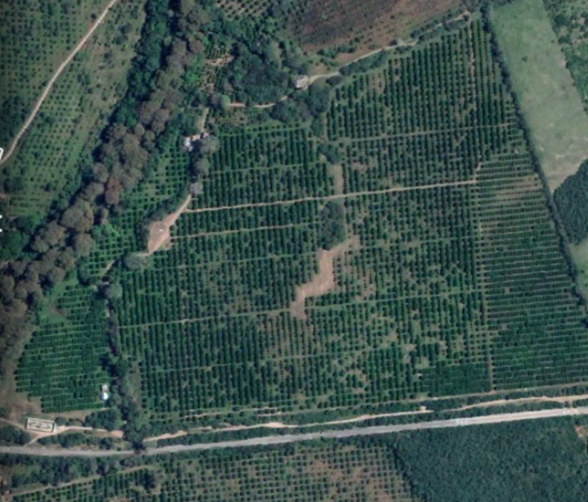
\includegraphics[width=0.5\textwidth,keepaspectratio=true]{images/C4/Huerta.png}
\caption{Plano cenital de una huerta en el estado de Tamaulipas.}
\end{figure}
La posición inicial de los psílidos no está basada en las observaciones de campo, pues comúnmente cuando éstos llegan a poblar un campo, se instalan en los árboles de los extremos de la huerta y difícilmente arriban a árboles más céntricos, sin embargo, como en este trabajo se resume el problema a una sola huerta, este hecho no tiene un efecto relevante, y el comportamiento de la enfermedad se torna más perceptible cuando más al centro se coloquen inicialmente los psílidos. Una vez colocados en algún punto aleatorio del campo, la distancia que suelen recorrer los psílidos en un día no rebasa algunos cuantos metros; cabe mencionar que los efectos del viento en la dinámica del insecto no ha sido considerada en este trabajo. La cantidad inicial que es colocada es arbitrariamente de 100 individuos, de los cuales el 15\% está infectado, su crecimiento se ha modelado por la función logística con una capacidad máxima en cada árbol de 300 centenas de insectos, esta capacidad máxima ha sido observada en campos en los que no se aplica control de la plaga. En el caso de esta simulación, dadas las dimensiones del campo y la capacidad máxima de cada árbol, la capacidad total de la huerta está por encima de las novecientas mil centenas. La probabilidad de contagio de un psílido que se alimenta del árbol, así como la probabilidad de transmisión de la bacteria en los psílidos infectados a los árboles sanos han sido calibradas para reproducir los niveles observados de árboles sintomáticos a través del tiempo. El tiempo de incubación se ha configurado para ser en promedio de 200 días, esta cantidad ha sido observada para al menos una especie de cítrico, y los valores se desvían de esta cantidad dentro de un entorno de ±50 días, aunque para algunos experimentos fueron probados entornos de distinto radio.

\begin{table}[!ht]
    \centering
    \begin{tabular}{|l|p{0.7in}|p{0.7in}|p{0.6in}|p{0.7in}|p{0.65in}|p{0.45in}|}
    \hline
        Nombre & Tiempo de \newline incubación\newline mínimo & Tiempo de\newline incubación\newline máximo & Per'ioodo\newline del\newline pesticida & Mortalidad\newline del\newline pesticida & Periodo de\newline revisión\newline y corte & Corte\newline de\newline vecinos  \\ \hline
        Control1 & 150 días & 250 días& Ninguno & Ninguno & Ninguno & No  \\ \hline
        Control2 & 165 días & 235 días& Ninguno & Ninguno & Ninguno & No  \\ \hline
        Control3 & 180 días& 220 días& Ninguno & Ninguno & Ninguno & No  \\ \hline
        Pesticida1 & 150 días& 250 días& 90 días& 50\%& Ninguno & No  \\ \hline
        Pesticida2 & 150 días& 250 días& 90 días& 70\%& Ninguno & No  \\ \hline
        Pesticida3 & 150 días& 250 días& 90 días& 90\%& Ninguno & No  \\ \hline
        Pesticida4 & 150 días& 250 días& 60 días& 70\%& Ninguno & No  \\ \hline
        Pesticida5 & 150 días& 250 días& 90 días& 70\%& Ninguno & No  \\ \hline
        Pesticida6 & 150días & 250 días& 180 días& 70\%& Ninguno & No  \\ \hline
        Corte1 & 150 días& 250 días& Ninguno & 70\%& 90 días& No  \\ \hline
        Corte2 & 150 días& 250 días& Ninguno & 90\%& 60 días& No  \\ \hline
        Corte3 & 150 días& 250 días& Ninguno & 70\%& 15 días& No  \\ \hline
        CorteVecinos & 150 días& 250 días & 90 días& 70\%& 90 días& Sí  \\ \hline
        PesticidaCorte & 150 días& 250 días& 90 días& 70\%& 90 días& Sí  \\ \hline
    \end{tabular}
\end{table}


\subsection{Pruebas principales con distintas variables}

%--------------------------------------------------------------------------------HORNADA PRINCIPAL

%Simulación de control
%Pesticida solo
%Corte individual
%Corte Vecinos
%Métodos conjuntos

La primera ejecución del código tiene el objetivo de servir como punto de referencia para las simulaciones próximas, por esta razón, los métodos de control han sido omitidos de tal forma que la plaga y la enfermedad puedan desarrollarse libremente. En esta y en las siguientes simulaciones, el tiempo medio de aparición de síntomas en árboles infectados es de 200 días a partir de su infección, este período de incubación puede tomar valores mínimos de 150 días y máximos de 250.
La segunda ejecución contempla el mismo escenario que la ejecución de control pero adhiere la aplicación periódica de pesticida cada noventa días, aproximadamente tres meses, que es el tiempo mínimo indicado por el protocolo. La mortalidad en la aplicación es del 70\%, que es el valor medio de la medida en los experimentos de campo, y es consistente con la información proporcionada por los fabricantes. La aplicación de pesticida es el único método de control de esta simulación.
La tercera ejecución, por otra parte, usa el método de control que consiste en una revisión periódica de todos los árboles de la huerta cada 60 días y el corte inmediato de los árboles que presenten síntomas de infección, este método es el único que se aplica en la tercera ejecución.
La cuarta ejecución es idéntica a la tercera salvo por el criterio para cortar árboles, dado que mientras que la tercera solamente corta al árbol con síntomas, en esta se talan también a los cuatro árboles contiguos al árbol sintomático.
Finalmente, las simulaciones quinta y sexta combinan los métodos usados en las simulaciones cuarta y segunda, con la diferencia de que en la simulación quinta el tiempo de revisión para tala es de noventa días mientras que en la sexta es de 15. Los métodos usados son una representación fiel de lo que se practica en los campos reales, el control en la población de psílidos y la eliminación de los árboles infectados y sus vecinos junto con los psílidos que contengan. Los resultados que retornaron son útiles para entenderlos.


%--------------------------------------------------------------------------------HORNADAS SECUNDARIAS SI SE NECESITASEN
%\subsection{Pruebas secundarias con distintas variables}
%Pruebas de control

%Aplicación de pesticidas sin tala
%Dureza del pesticida(50%, 70%, 90%)a 3 meses

%Período del pesticida(6meses, 3 meses, 2 meses)con el 70%

%Tala de árboles sin pesticidas
%   Individual
%Tiempo de vigilancia(90, 60 y 15 días)

%   Con vecinos
%a 90 días

%Métodos de control conjunto
%3 meses 70%